\section[Magnetisches Verhalten von Aluminium]{Einfluss eines Magneten auf eine Aluminiumplatte und auf einen Aluminiumkamm }\label{kap:Kamm_Platte}
Bei diesem Experiment ging es darum das verhalten zweier unterschiedlich geformter Körper aus dem gleichem Material zu untersuchen. Der Versuchsaufbau ist in \cref{fig:Alukamm} zu sehen.
Um das verhalten der Platte und des Kammes zu untersuchen wurde eine Reihe aus drei Magneten  auf die Platte zubewegt und entfernt. Diese Aktionen wurden danach bei dem Kamm wiederholt.
Beim schnellen annähern an die Platte schwang die Platte zurück und beim langsamen entfernen wurde sie mitgezogen.
Dieses verhalten ist auf Diamagnetismus beziehungsweise Paramagnetismus zurückzuführen. Beim annähern tritt zunächst ein Paramagnetischer Effekt auf und die Platte wird von dem Magneten angezogen. Doch sobald der Magnet der Platte zu nah kam wurde die Platte zurückgestoßen was auf diamagnetische Effekte zurückzuführen ist. Entfernt man die Magneten jedoch langsam wieder überlagern die deutlich stärkeren Paramagnetischen Effekte den Diamagnetismus und die Platte wird mitgezogen.
Das dass Magnetische verhalten der Platte sich änderte ist dadurch zu erklären das diamagnetische Effekte in einem Starken Magnetfeld alle anderen Effekte überlagern. Genau dies passierte beim annähern an die Platte.
Bei dem Kamm waren diese Diamagnetischen Effekte nicht zu beo0bachten und auch die Paramagnetischen Effekte wurden nur sehr schwach beobachtet. Der Grund für dieses Verhalten ist bei den Unterbrechungen der Oberfläche zu  suchen, da dies der einzige unterschied vom Kamm zur Platte ist. Diese Unterbrechungen sorgen dafür das die Wirbelströme, die auf die Oberfläche induziert werden deutlich schwächer ausfallen als bei der Platte.
Dadurch wird der sowieso schon sehr schwache Diamagnetische Effekt so stark abgeschwächt das er bei einem so schwachen Magnetfeld nicht mehr zu sehen ist.
\begin{figure}[h]
	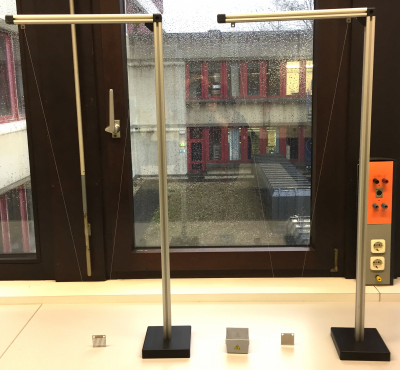
\includegraphics[width=0.5\textwidth]{res/Alupendel.png}
	\caption{In dieser Abbildung ist der Versuchsaufbau zu sehen mit dem man den Einfluss eines Magneten auf eine Aluplatte und auf einen Alukamm untersucht wurde\protect\footnotemark.}
	\label{fig:Alukamm}
\end{figure}
\footnotetext{Entnommen am 20.11.17  aus dem Learnweb Kurs "Experimentelle Übungen I 17-18"}
